\chapter{Fundamentos Teóricos}
El presente capítulo abarca los principales temas que se abordan a lo largo de la investigación. Se detalla qué es un sistema de capacitación automatizado, su importancia, sus tipos de preguntas y los modelos de calificación que siguen. Además, se plantea el concepto de sistemas expertos, junto a sus características más notables y su importancia. También estarán explicadas algunas de las funcionalidades del Sistema de Entrenamiento SECPROIT, sus componentes y rendimiento.
Al final del capítulo se observan conclusiones parciales a modo de resumen del mismo.

\section{Sistemas de Capacitación Automatizados}
La capacitación laboral es un método aplicado por las empresas para que su personal adquiera nuevos conocimientos profesionales. Por lo general, se produce ante un ascenso o incorporación, aunque no son los únicos motivos. Lo ideal es que se desarrolle de forma continúa, ya que la constante formación del personal deriva en resultados positivos tanto para el grupo de trabajo como para la organización en la que se realiza \cite{blogBizneo}.
Surge en el mundo como respuesta a la necesidad de mejorar permanentemente la calidad y formación de recursos humanos.

Basándose en el concepto anterior, un sistema de capacitación automatizado, también conocido como sistema de entrenamiento, es un método de enseñanza alternativo creado para el adiestramiento de los trabajadores. Se basa, principalmente, en un software que permite el aprendizaje de los usuarios sin necesidad de una supervisión constante. Generalmente, resulta más efectivo que las prácticas de enseñanza presencial, debido a que el estudiante trabaja solo y puede determinar su propia velocidad de aprendizaje, usando una amplia variedad de herramientas y métodos para la transferencia del conocimiento \cite{seguridadMinera}.

A modo de resumen, es un software que brinda una solución de recursos humanos, ayuda en la formación de los trabajadores y aumenta la productividad empresarial.

\subsection{Características de un Sistema de Capacitación}
Un sistema de capacitación, ya sea automatizado o no, ofrece diferentes aplicaciones en función del modelo de negocio que utiliza. Su versatilidad permite adaptarse a las necesidades particulares de cada sector. Sin embargo, según \cite{softDoit}, la mayoría de los sistemas contienen las mismas características:
\begin{itemize}
\item Son capaces de gestionar los distintos cursos impartidos, la asistencia y la inversión en formación de la empresa.
\item Asignan a los empleados que deberán asistir y los profesionales responsables de analizar sus resultados.
\item Detectan las carencias formativas del personal antes de que influyan en el desarrollo del trabajo.
\item Clasifican las distintas actividades formativas en base a su categoría y catálogo.
\item Registran y consultan el progreso del aprendizaje de los empleados en tiempo real.
\end{itemize}

\subsection{Importancia de los Software de Capacitación}
Un sistema de entrenamiento asistido por computadora permite ofrecer el mismo nivel de adiestramiento para cada usuario del sistema, en cuanto a rigor y evaluación. Uno de los problemas de la capacitación de los empleados de manera presencial, es que las sesiones son frecuentemente inconsistentes, y las diferencias en el nivel de habilidad del formador pueden tener un impacto significativo en el éxito del empleado. Al contar con un sistema automatizado, solo se necesita una base de conocimientos para garantizar el mismo nivel de entrenamiento para todos los capacitados \cite{cap2002}.

\subsection{Fases de un Proceso de Evaluación de Conocimiento}
Un proceso de evaluación de conocimiento, debe estar integrado por cinco etapas (Figura \ref{fig:etapasEval}), asegura \cite{garcia1994}. Cada una de ellas, va a marcar un conjunto de acciones, que al final se interpretarán como un buen entrenamiento:

\begin{itemize}
\item \textsl{Recogida de Datos:} es la recopilación sistemática de toda la información a lo largo del proceso completo de enseñanza-aprendizaje. Debe tener concordancia con los objetivos, ser suficiente, representativa, relevante y ponderada, en función del peso otorgado a cada objetivo. En los sistemas en línea estas posibilidades de registrar evidencias son inmensas.
\item \textsl{Puntuación de las Pruebas:} se realiza una vez medidos, de manera cuantitativa o cualitativa, los distintos bloques de información, con las ponderaciones, criterios e indicadores que se hayan establecido.
\item \textsl{Juicio de Valor:} puede hacerse limitándose a criterios de grupo (evaluación normativa), refiriéndose a criterios de superación de objetivos y/o contenidos (evaluación de criterio), o teniendo en cuenta la personalidad, posibilidades y limitaciones del propio sujeto del aprendizaje (evaluación personalizada).
\item \textsl{Toma de Decisiones:} habitualmente denominada calificación, trae consigo una serie de consecuencias personales, administrativas, económicas y laborales. Se basa en la decisión a partir del resultado. La acción resultante influye directamente en el adiestrado. Ejemplos de decisiones son: selección/exclusión, promoción/recuperación/repetición, rebajar a niveles anteriores, ampliación, certificación/reprobación, entre otras.
\item \textsl{Información a los Interesados:} es la etapa final, que ha de llegar a diferentes destinatarios, aunque principalmente y de forma adecuada, a los capacitados. Es la confirmación de que concluye el entrenamiento.
\end{itemize}

\begin{figure}[h]
\centering
 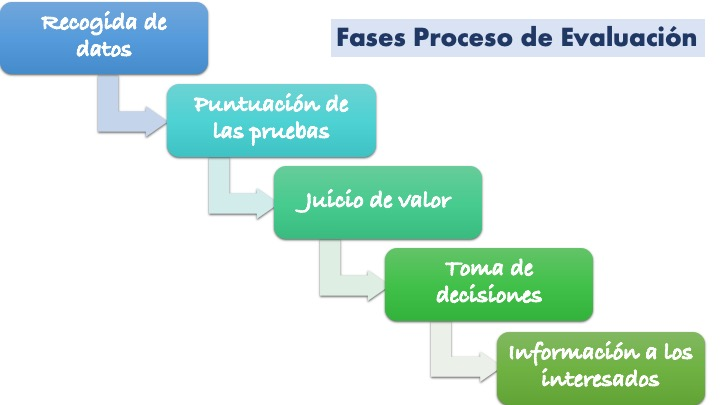
\includegraphics[width=0.5\linewidth]{imagen/FasesEva.jpg}
 \caption{Etapas para garantizar un buen Sistema de Capacitación.}
 \label{fig:etapasEval} 
\end{figure}

\subsection{Tipos de Preguntas en un Sistema de Capacitación Automatizado}
A medida que avanza el tiempo, se generan nuevos métodos de estudio, y con estos, nuevas formas de preguntar y calificar. Sin embargo, a la hora de diseñar un sistema automatizado, no es menos cierto que existen algunas variantes más sencillas y por ende, más utilizadas. Según \cite{referencia12} los tipos de preguntas que mayormente se emplean en un sistema de este tipo son:
\begin{itemize}
\item \textsl{Verdadero o Falso:} contienen una declaración que se debe indicar si es verdadera o no. Permiten responder en poco tiempo, son fáciles, rápidos de calificar y se corrigen de forma automática.
\item \textsl{Opción Múltiple:} se componen de una pregunta (raíz) con
múltiples respuestas posibles. Pueden incluir múltiples opciones válidas, en cuyo caso, podrían darse por superada al marcar cualquiera de ellas o cuando se marquen todas. Se caracterizan por ser fáciles y rápidas de calificar, se
corrigen automáticamente y se pueden utilizar para evaluar los conocimientos en una amplia gama de contenidos.
\item \textsl{Emparejar, Relacionar u Ordenar:} por lo general se emparejan cada una de las opciones del primer bloque con las opciones dadas en el segundo bloque, o se ordenan bloques de modo que quede una secuencia correcta de acuerdo a un patrón previamente establecido. Se suelen usar en aquellos cursos donde la adquisición de conocimientos muy detallados es un objetivo importante. Son preguntas fáciles de diseñar, rápidas de calificar y se corrigen
automáticamente. Estadísticamente, se tarda más en responder que las preguntas anteriores.
\item \textsl{Respuesta Corta:} basta con que se escriban un par de palabras o una frase sencilla. Una alternativa más común a este tipo de preguntas es la de cubrir espacios en blanco con una palabra. Este tipo de preguntas son muy útiles para que se demuestren los conocimientos basados en hechos o palabras claves. La dificultad para calificarlas depende del estilo que se decida emplear.
\end{itemize}

\subsection{¿Cómo verificar la validez de las respuestas?}
Una vez terminado el entrenamiento, mediante el proceso de evaluación, se debe comprobar cuáles de los resultados obtenidos son correctos y cuáles no. Para ello se deben comparar las respuestas del evaluado con una fuente de confianza, que contenga la información verídica de lo que se está tratando. Estas fuentes de confianza se conocen por el nombre: bases de conocimiento.
A partir de ellas, se verifica si los datos en las respuestas del evaluado coinciden con la información real contenida en la base. Este proceso puede realizarse tanto de manera manual, semi-automática o automática \cite{Christmann2022}.

Al tratarse de un sistema de capacitación automatizado, por lo general, el método utilizado para validar las respuestas es el automático. De esta forma se facilita el trabajo para aquellos que deben evaluar a un personal abundante. Según \cite{AltyJL1984}, la manera más efectiva y eficiente de evaluar estos sistemas es a partir del uso de un Sistema Experto.

\subsection{¿Cómo se evalúa una Capacitación?}
La evaluación y la calificación de una prueba, no pueden depender de un solo instrumento o técnica, ya que de esa forma solo se mide un tipo de aprendizaje. Los criterios para calificar que se designen, serán los porcentajes de valor que se establezcan a cada resultado de las actividades realizadas y a su resultado final. Se debe tomar en cuenta tanto la exactitud de la respuesta, como el proceso que se siguió para llegar a la misma, así como la cantidad de intentos necesarios utilizados para hallar la solución correcta.
Una evaluación posee dos objetivos principales: analizar en qué medida se han cumplido los objetivos, para detectar posibles fallas en el proceso y poder superarlas, y proporcionar la reflexión de los que realizaron el entrenamiento en torno a su propio proceso de aprendizaje (metacognición) \cite{RonaldL.Jacobs2012}.

A modo de resumen, para realizar una correcta evaluación se deben tener en cuenta tantas herramientas como parámetros influyan. En este caso en particular: la puntuación de las respuestas y la cantidad de intentos.

%%%%%%%%%%%%%%%%%%%%%%%%%%%%%%%%%

\section{Sistemas Expertos}
Los sistemas expertos resuelven problemas que normalmente son solucionados por expertos humanos. Para resolverlos, necesitan acceder a una importante base de conocimiento sobre el dominio, que debe construirse de la manera más eficiente posible.
Utilizan uno o más mecanismos de razonamiento, para aplicar este conocimiento a los problemas que se le proponen. Cuentan con un mecanismo para explicar a los usuarios que han confiado en ellos, lo que han hecho \cite{AltyJL1984}.

Una forma de contemplar los sistemas expertos es que representan la mayor parte de la Inteligencia Artificial (IA) aplicada. Un sistema experto en IA se define como un programa informático que tiene la capacidad de representar y razonar sobre el conocimiento \cite{Rasheed2021}.

\subsection{Componentes de un Sistema Experto}
En \cite{OdhiamboOmuya2021} se comentan los diferentes componentes que integran un sistema experto. Aunque pueden contar con un número mayor de componentes, los mínimos requeridos son (Figura \ref{fig:componentesSE}):

\begin{itemize}
\item \textsl{Motor de Inferencia:} es el corazón del sistema experto. Su cometido principal es sacar conclusiones aplicando el conocimiento a los datos. Estas conclusiones pueden estar basadas en conocimiento determinista o conocimiento probabilístico.
\item \textsl{Base de Conocimientos:} consiste en un conjunto de objetos y un conjunto de reglas, que gobiernan las relaciones entre esos objetos. La información que almacena es de naturaleza permanente y estática, es
decir, no cambia de una aplicación a otra. Se debe diferenciar entre los datos y
el conocimiento. El conocimiento se refiere a afirmaciones de validez general tales como reglas, distribuciones de probabilidad, entre otras. Los datos se refieren a información relacionada con una aplicación en particular \cite{Potapova2021}.
\item \textsl{Mecanismo de Aprendizaje:} controla el flujo del nuevo conocimiento que va del experto humano a la base de conocimiento. El sistema determina qué nuevo conocimiento se necesita, o si el conocimiento es realidad, es decir, si debe incluirse, y en caso necesario incorporar dicho
conocimiento.
\item \textsl{Interfaz de Usuario:} se constituye como la interfaz entre el sistema experto y el usuario. Para que sea efectiva debe incorporar mecanismos para mostrar y obtener información de forma sencilla y agradable.
\end{itemize}

\begin{figure}[h]
\centering
 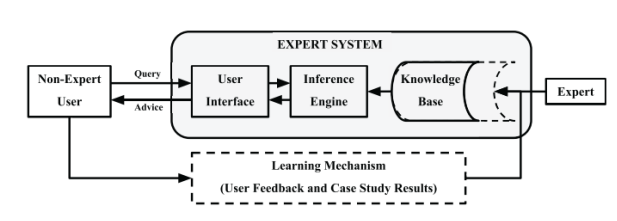
\includegraphics[width=0.5\linewidth]{imagen/ComponentesSE.png}
 \caption{Componentes mínimos requeridos en un Sistema Experto.}
 \label{fig:componentesSE} 
\end{figure}

\subsection{Ventajas de un Sistema Experto}
El uso de un sistema experto en cualquier ámbito social, resulta favorable de diversas maneras. En \cite{KandulaNeha2020} se mencionan algunas de estas ventajas:

\begin{itemize}
\item Mientras que un experto humano tiene limitaciones y percances propias de su condición humana, el Sistema Experto no sufre de estas cuestiones y se convierte en una herramienta estable y fiable para su entorno.
\item Sus actividades son completamente replicables y siempre contesta de la misma manera a menos que se le cambie el diseño.
\item La velocidad de procesamiento es mayor al de un ser humano.
\item Debido a la escasez de expertos humanos en determinadas áreas, los sistemas expertos pueden almacenar su conocimiento para cuando sea necesario aplicarlo.
\item Pueden ser utilizados por personas no especializadas para resolver problemas.
\item Pueden ser usados como sistema de aprendizaje.
\item Si se evalúa el costo total del empleo de esta tecnología, la replicabilidad y estabilidad, asociado a la seguridad que provee, resulta una ecuación favorable, aun considerando que las inversiones iniciales pueden ser
relativamente elevadas.
\end{itemize}

\subsection{Desventajas de un Sistema Experto}
A su vez, el empleo de estos sistemas puede traer consigo alguna desventaja. Nuevamente, en \cite{KandulaNeha2020} se mencionan algunas de estas:

\begin{itemize}
\item Para actualizarlos se necesita de reprogramación, siendo una de sus limitaciones más acentuadas.
\item Poseen elevado costo en dinero y tiempo, además que estos programas son poco flexibles a cambios y de difícil acceso a información no estructurada.
\item Carecen de sentido común, para un sistema de este tipo no hay nada obvio.
\item No podemos mantener una conversación informal con estos sistemas.
\item Para un sistema experto es muy complicado aprender de sus errores o de errores ajenos.
\item No son capaces de distinguir cuales son las cuestiones relevantes de un
problema y separarlas de cuestiones secundarias.
\end{itemize}

Sin embargo, estos problemas no solo los presentan los sistemas expertos, puesto que la inteligencia artificial aún no ha podido desarrollar sistemas que
sean capaces de resolver problemas de manera general o de aplicar el sentido común para resolver situaciones complejas o controlar situaciones ambiguas. Es por eso que, a pesar de sus desventajas, los sistemas expertos son considerados una gran ayuda y un enorme avance, en especial, en los sistemas de capacitación.

\subsection{¿Por qué usar un Sistema Experto en este Entrenador?}
La Industria Alimentaria Cubana trabaja de manera ininterrumpida, con un personal laboral que cambia frecuentemente. Es por ello que no cuentan con la cantidad de expertos necesarios para que se atiendan, de manera constante, todos los procesos que en ella ocurren. La capacitación presencial de los trabajadores no es una opción válida, puesto que sufren de constante cambio de personal y los expertos no poseen el tiempo para capacitarlos a todos. Por estas razones, se hace imprescindible la tarea de entrenar, de alguna manera, a los operarios de esta industria, ya que lográndolo, se garantiza una mejor respuesta ante una falla en algún proceso productivo \cite{gestorBases}.

Un método muy eficiente para entrenar a este personal, es mediante un sistema de capacitación digital, porque, como bien se fundamentó en la sección anterior, así pueden aprender por sí solos, sin la presencia de un experto y a su propio ritmo, y pueden ser evaluados de las mismas maneras, sin distinciones de preferencias o errores humanos. Con una capacitación digital también se logra hacer más sencillo el trabajo del jefe de área, ya que solo deberá seleccionar al mejor entre un conjunto de resultados, sin tener que aplicar pruebas o entrevistas.

Los procesos que se manejan en esta industria se caracterizan por tener datos estructurados en variables, donde cada variable tiene sus características principales, las causas que pueden volverla inestable y las recomendaciones a seguir para que no ocurra un incidente o qué hacer en caso de que ya ocurriese. Este grupo de datos conforma una base de conocimientos.

Si se analiza en conjunto los datos que se tienen y las necesidades que se desean cumplir, se llega a la conclusión de que se quiere crear un sistema de entrenamiento, para capacitar a un conjunto de trabajadores debido a la ausencia de expertos humanos, y para ello se cuenta con una base de conocimientos y un mecanismo de aprendizaje diseñado. A modo de resumen, un sistema experto.

%%%%%%%%%%%%%%%%%%%%%%%%%%%%%%%%%

\section{Sistema de Entrenamiento SECPROIT}
Para brindar una solución a la principal problemática de esta investigación, en el año 2018 se crearon dos aplicaciones que trabajarían de manera conjunta. La primera es un Gestor de Bases de Conocimientos que permite crear las bases de información que se necesitan para evaluar a los trabajadores. La segunda es conocida como Sistema Experto para el Control de Procesos Químicos (SECPROIT), que es un sistema diseñado para capacitar a los operarios de las fábricas. Ambos sistemas fueron desarrollados en la Universidad Tecnológica de La Habana José Antonio Echeverría (CUJAE), entre las facultades de Ingeniería Química e Ingeniería Informática. Ambas aplicaciones sirvieron para defender el título de Ingeniería.

Aunque estas aplicaciones se encuentren estrechamente vinculadas a este trabajo, en la mismo se abordará más, el sistema SECPROIT. El objetivo principal es lograr un sistema semejante con mejores prestaciones y funcionalidades, una actualización.

\subsection{¿Cómo funciona el SECPROIT?}
En el sistema existen tres roles fundamentales: el administrador que se encarga de llenar los datos de los usuarios, el especialista que inserta los procesos para los entrenamientos y supervisa los resultados obtenidos por los trabajadores de su área laboral, y el operario que realiza la capacitación. Cada usuario tiene un nombre y una contraseña, y con cada rol aparecen funcionalidades únicas. Un rol no puede realizar las acciones de otro.

En el caso de los especialistas, deben registrar de cada proceso el nombre, una imagen si la posee, un fichero tipo \textsl{anm} y un archivo \textsl{drl}. Los ficheros \textsl{anm} contienen los nombres de todas las variables que influyen en el proceso, las características, todas las causas que pueden afectar el proceso y todas las recomendaciones para todas las causas descritas. El archivo \textsl{drl} contiene las reglas que enlazan las variables con sus causas y las causas con sus recomendaciones. Dichas reglas siguen una estructura específica: comienza con un patrón para el nombre de la regla, luego presenta los posibles atributos que posee, la sentencia que se debe cumplir y las acciones que realizar si se cumple la sentencia (Figura \ref{fig:drools}). Este archivo es lo que se conoce como Motor de Reglas (\textsl{Drools}). Esta información es extraída del sistema Gestor de Bases de Conocimientos \cite{anaMailen}.

\begin{figure}[h]
\centering
 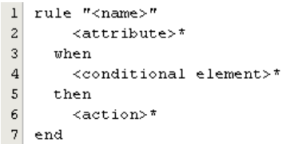
\includegraphics[width=0.5\linewidth]{imagen/EstructuraDRL.png}
 \caption{Estructura de un archivo \textsl{drl}.}
 \label{fig:drools} 
\end{figure}

Por su parte, el operario entrará a realizar aquellos entrenamientos que el especialista haya validado. Una vez comenzado, deberá señalar, de un grupo de variables, las que por su estado estén en peligro de inestabilidad. Si ha seleccionado correctamente pasa a la siguiente etapa, donde debe escoger qué causa el estado de las variables que prefirió. Por último deberá seleccionar qué recomendaciones seguir para cada causa que señaló. Este entrenamiento es un proceso continuo donde, si decides abandonar sin haber terminado, no se guardarán los cambios y aparecerá como prueba no superada. La puntuación está dada de manera genral, como porcentaje entre las notas de las tres etapas \cite{elena}.

\subsection{Limitaciones Actuales del Sistema}
Actualmente el sistema posee ciertas limitaciones que afectan la experiencia de usuario, así como el disfrute de la aplicación. También encontramos algunas en sus principales funcionalidades:

\begin{itemize}
\item Los entrenamientos de un proceso son únicos, es decir, solo se evalúa ese contenido una vez, sin brindar la posibilidad de mejorar o aprender.
\item Las etapas del entrenamiento son continuas, sin posibilidad de pausa o descanso.
\item Si no se aprueba una de las etapas del entrenamiento, el operario deberá continuar y concluirlo, aunque ya esté suspenso.
\item En la última etapa de evaluación (escoger las recomendaciones), no se muestran los errores cometidos o el resultado obtenido.
\item La nota final está dada de manera general (aprobado o no) sin hacer énfasis en los errores cometidos.
\item No presenta una interfaz de usuario intuitiva.
\item El usuario debe realizar numerosos toques en pantalla para completar una acción y, debido a que el sistema se utilizará en personas de avanzada edad, dificulta el manejo del sistema.
\item Los colores del sistema son muy oscuros, lo que provoca que el usuario niegue la experiencia.
\end{itemize}

\subsection{Nuevas Acciones Sugeridas}


%%%%%%%%%%%%%%%%%%%%%%%%%%%%%%%%%

\section{Conclusiones del Capítulo}